\section{Simulation results with profiled data}
\label{sec:simResults}

To simulate the closed loop performance of the robot using the vanishing point algorithm for feedback, we implemented the robot dynamics, vanishing point measurements and control in Simulink. Since the execution time of the vanishing point algorithm is a delay to the controller, we also model the delay and power consumption for the vanishing mode chosen by the supervisory algorithm as a time varying delay to the input of the controller based on the profiled experimental data. With a setup similar to that shown in Fig. \ref{fig:juicyj}, we can accurately simulate both the closed loop behaviour of the system as well as the schedules, frequencies and power consumption of the computation platform.

For the simulations, we initialize the robot aligned to the corridor $\theta=0$ but off from the center by 0.25m, i.e. $x=0.25$. Note, velocity ($v$) is a constant parameter in our simulations. The controller will now attempt to bring the robot to the middle of the corridor and align it with the corridor while the supervisor decides the hardware operating mode ($\sigma,F_c,F_g$) for the vanishing point algorithm based on the online optimization of Sec. \ref{sec:scheduling}. At a simulation time of 10 seconds, we perturb the system with a steering disturbance which is a pulse of magnitude 3 degrees per second and a duration of 2 seconds. The controller again tries to recover from this disturbance while the supervisor picks the best operating mode for the perception algorithm. Since the controller's objective is to bring the robot to the middle of the corridor and keep it there (i.e. align it with the corridor), the closed loop control performance can be measured for a simulation time of $T$ seconds as follows

\begin{equation}
L = \int_0^T |x(t)|dt
\label{eq:ControlPerf}
\end{equation}

Also, the expected energy consumed by the computation platform can be achieved by simply integrating the expected power based on the selected operating mode of the algorithm during each time step. We evaluate the closed loop system to obtain these two metrics for a) the highest power (lowest delay) fixed operating mode, b) the lowest power (highest delay) fixed operating mode c) With switching between different modes based on the optimization of Eq.\ref{eq:cost_runtime} and the three functions for choosing $\alpha(t)$ as in Eqs \ref{eq:f1}, \ref{eq:f2}, \ref{eq:f3}. Figs. \ref{fig:cpuf} and \ref{fig:gpuf} show the selected CPU and GPU frequency versus time respectively. Fig. \ref{fig:power} show the computation power vs time, while Fig. \ref{fig:schedule} shows the schedule $\sigma$ of CPU-GPU allocation for tasks.


For these 5 cases, Fig. \ref{fig:xvst} shows the trajectory of $x$ versus time.  It is worth nothing that only the trajectory of $x$ for the lowest power, or highest delay mode differs significantly enough from the others so as to be different visually in this plot.


\begin{figure}[hbtp]
\centering
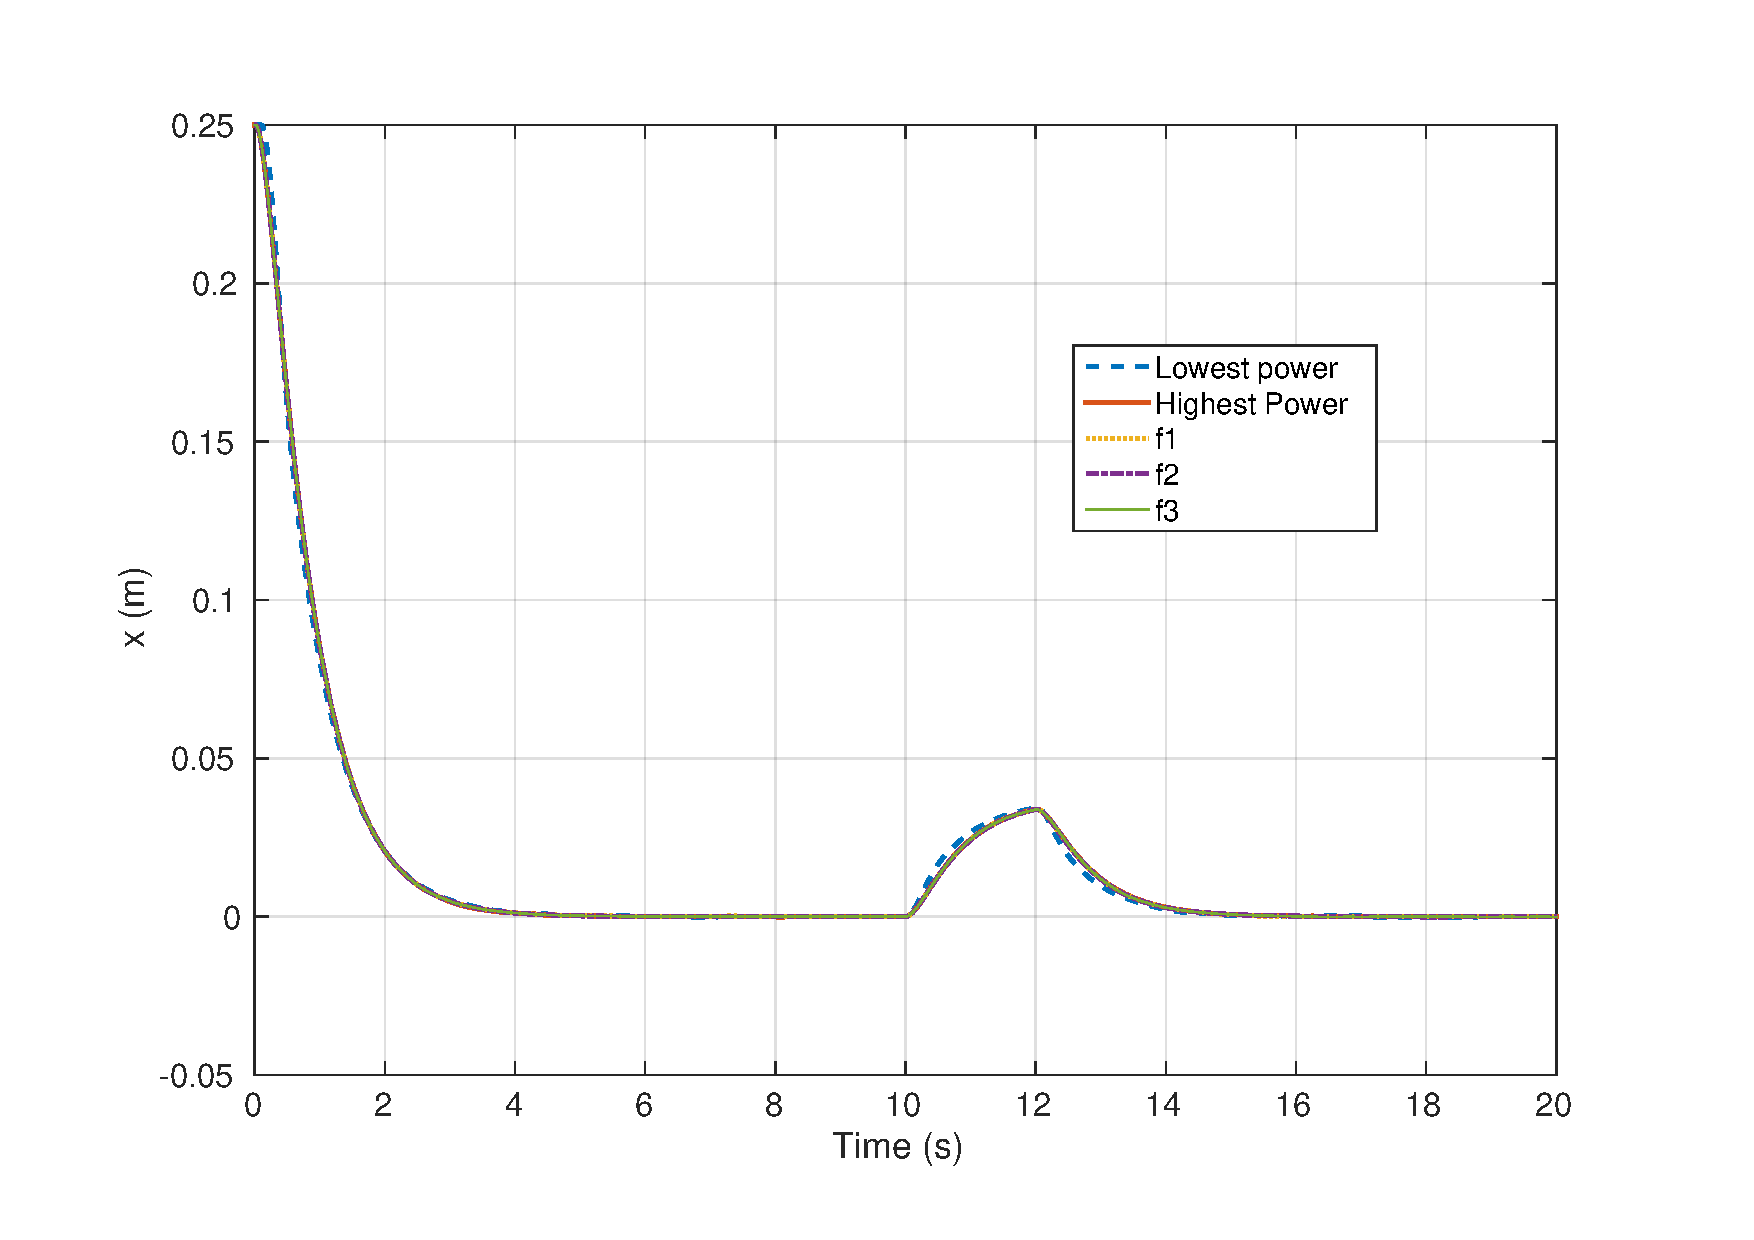
\includegraphics[width=0.49\textwidth]{../simulations/figs/xvst.pdf}
\caption{x position of the robot. Note, for modes other than the lowest power (most delay), the trajectory of x is very similar. This is also shown in table \ref{tbl:performance}}.
\label{fig:xvst} 
\end{figure}



To better understand these figures, let us go through 5 checkpoints (\textbf{a}, \textbf{b},\textbf{c}, \textbf{d} and \textbf{e}) in time common to Figs. \ref{fig:xvst}, \ref{fig:cpuf}, \ref{fig:gpuf}, \ref{fig:schedule} ,\ref{fig:power}.
At checkpoint \textbf{a} the controller starts to stabilize $x$ initial displacement of 0.25m. At this time, both $x_v$ and $x_m$ have high magnitudes, implying $\alpha$ takes a high value (close to 1) for all $f_i,\text{ }i=1,2,3$. Due to this, fig. \ref{fig:schedule} shows that $\sigma$ becomes $CCG$ and Figs. \ref{fig:cpuf} and \ref{fig:gpuf} show that CPU and GPU frequencies are high, this implies the vanishing point algorithm is near its highest throughput. Correspondingly, Fig. \ref{fig:power} shows that the computation power is also high.

At checkpoint \textbf{b} $x$ has a small magnitude and is near settling the middle of the corridor. Because of this, both $x_v$ and $x_m$ have smaller magnitudes, and so $\alpha$ is small and the requested CPU and GPU frequencies start to decrease. $\sigma$ is still $CCG$ for all supervisory functions except $f_2$, but settles to $CCC$ for all 3 as $x$ settles to zero shortly after checkpoint \textbf{b}.

Checkpoints \textbf{c}, \textbf{d}, and \textbf{e} show how the system responds to a pulse like disturbance in the steering (lasting from 10s to 12s) and settles (centers and aligns to the corridor) afterwards. It is interesting to see how the different supervisory functions $f_i$ result in different switching between schedule $\sigma=CCC$ and $\sigma=CCG$ and different CPU and GPU frequencies.




 
\begin{figure}[hbtp]
\centering
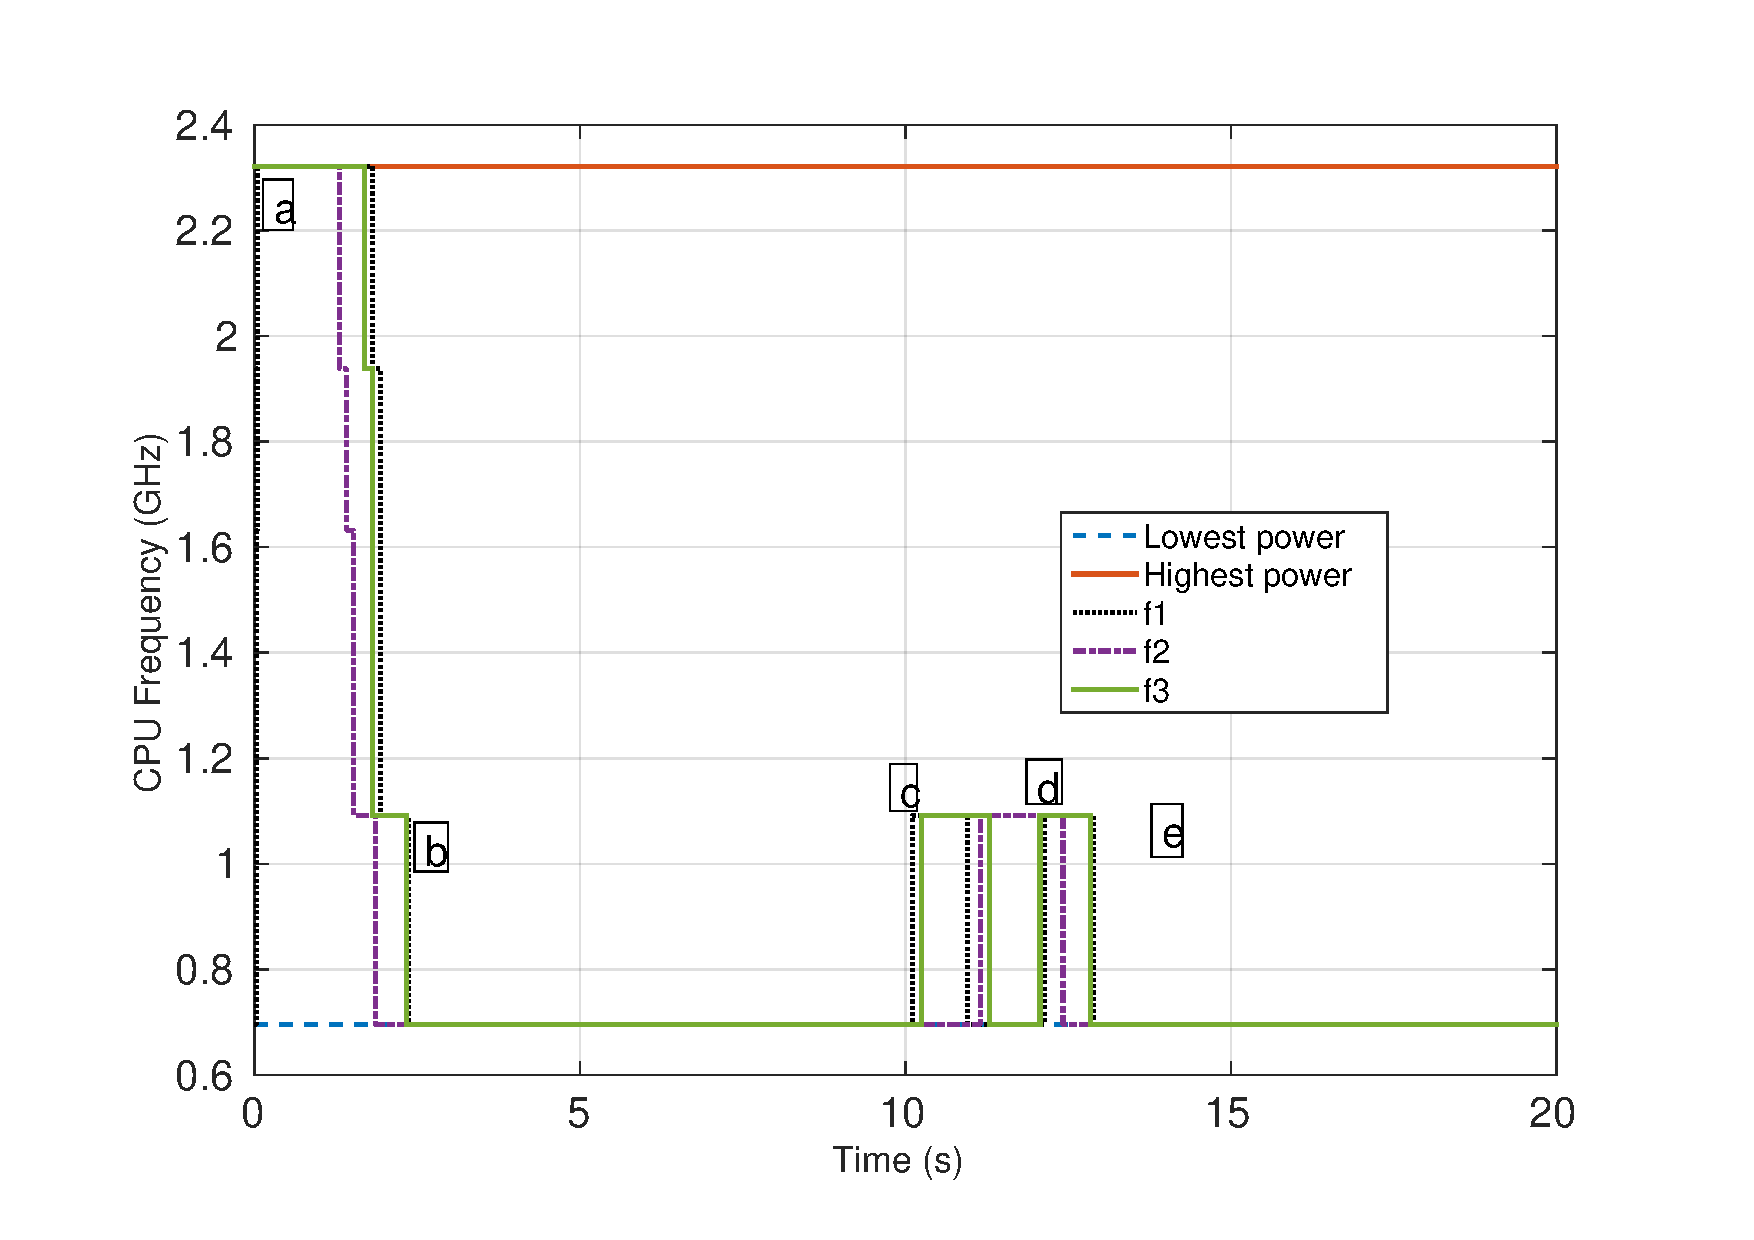
\includegraphics[width=0.49\textwidth]{../simulations/figs/CPUF.pdf}
\caption{CPU Frequency selected versus time.}
\label{fig:cpuf} 
\end{figure}


\begin{figure}[hbtp]
\centering
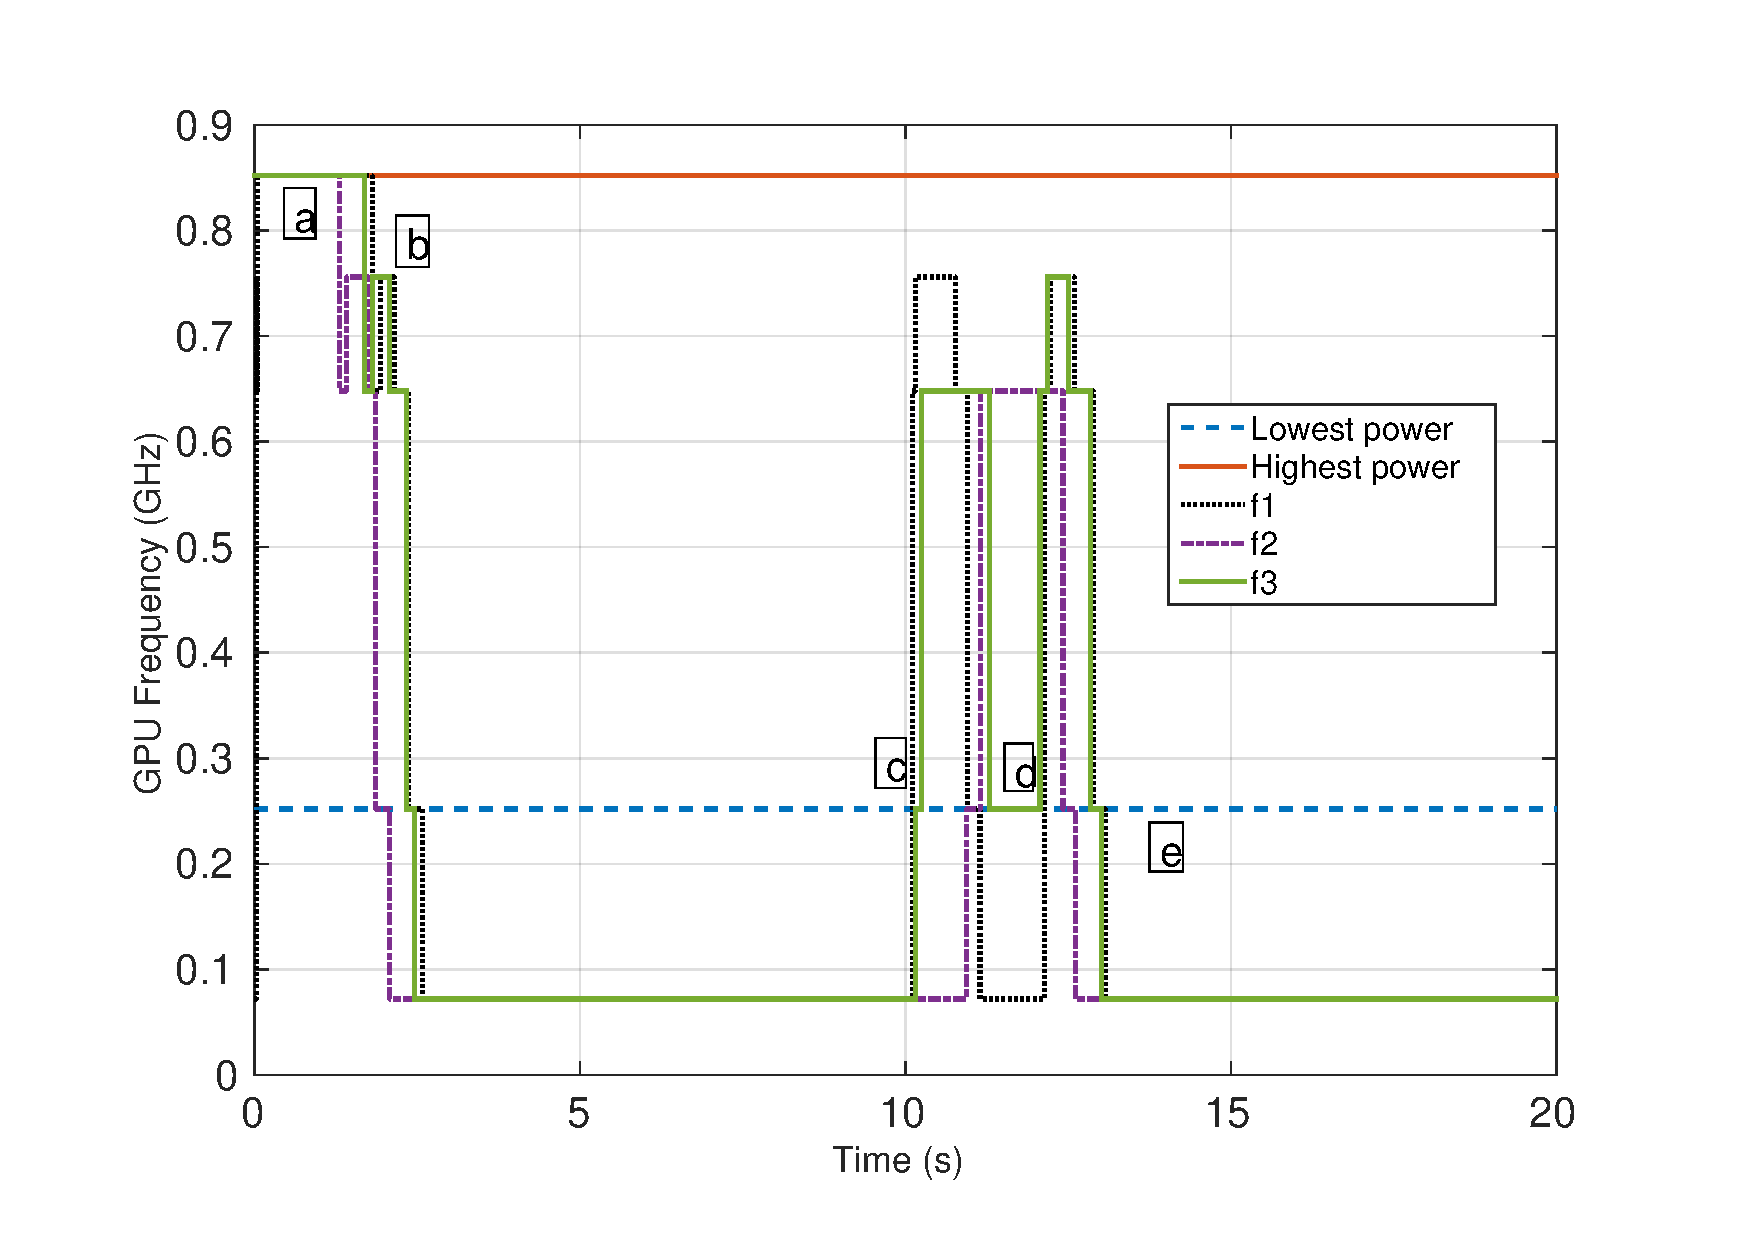
\includegraphics[width=0.49\textwidth]{../simulations/figs/GPUF.pdf}
\caption{GPU Frequency selected versus time. Note, for the lowest power mode, the GPU is at its second lowest frequency and not the lowest (while the schedule is $\sigma=CCC$). This is because of the noise in power data while the GPU frequency is being changed while it is not computing any tasks.}
\label{fig:gpuf} 
\end{figure}


\begin{figure}[hbtp]
\centering
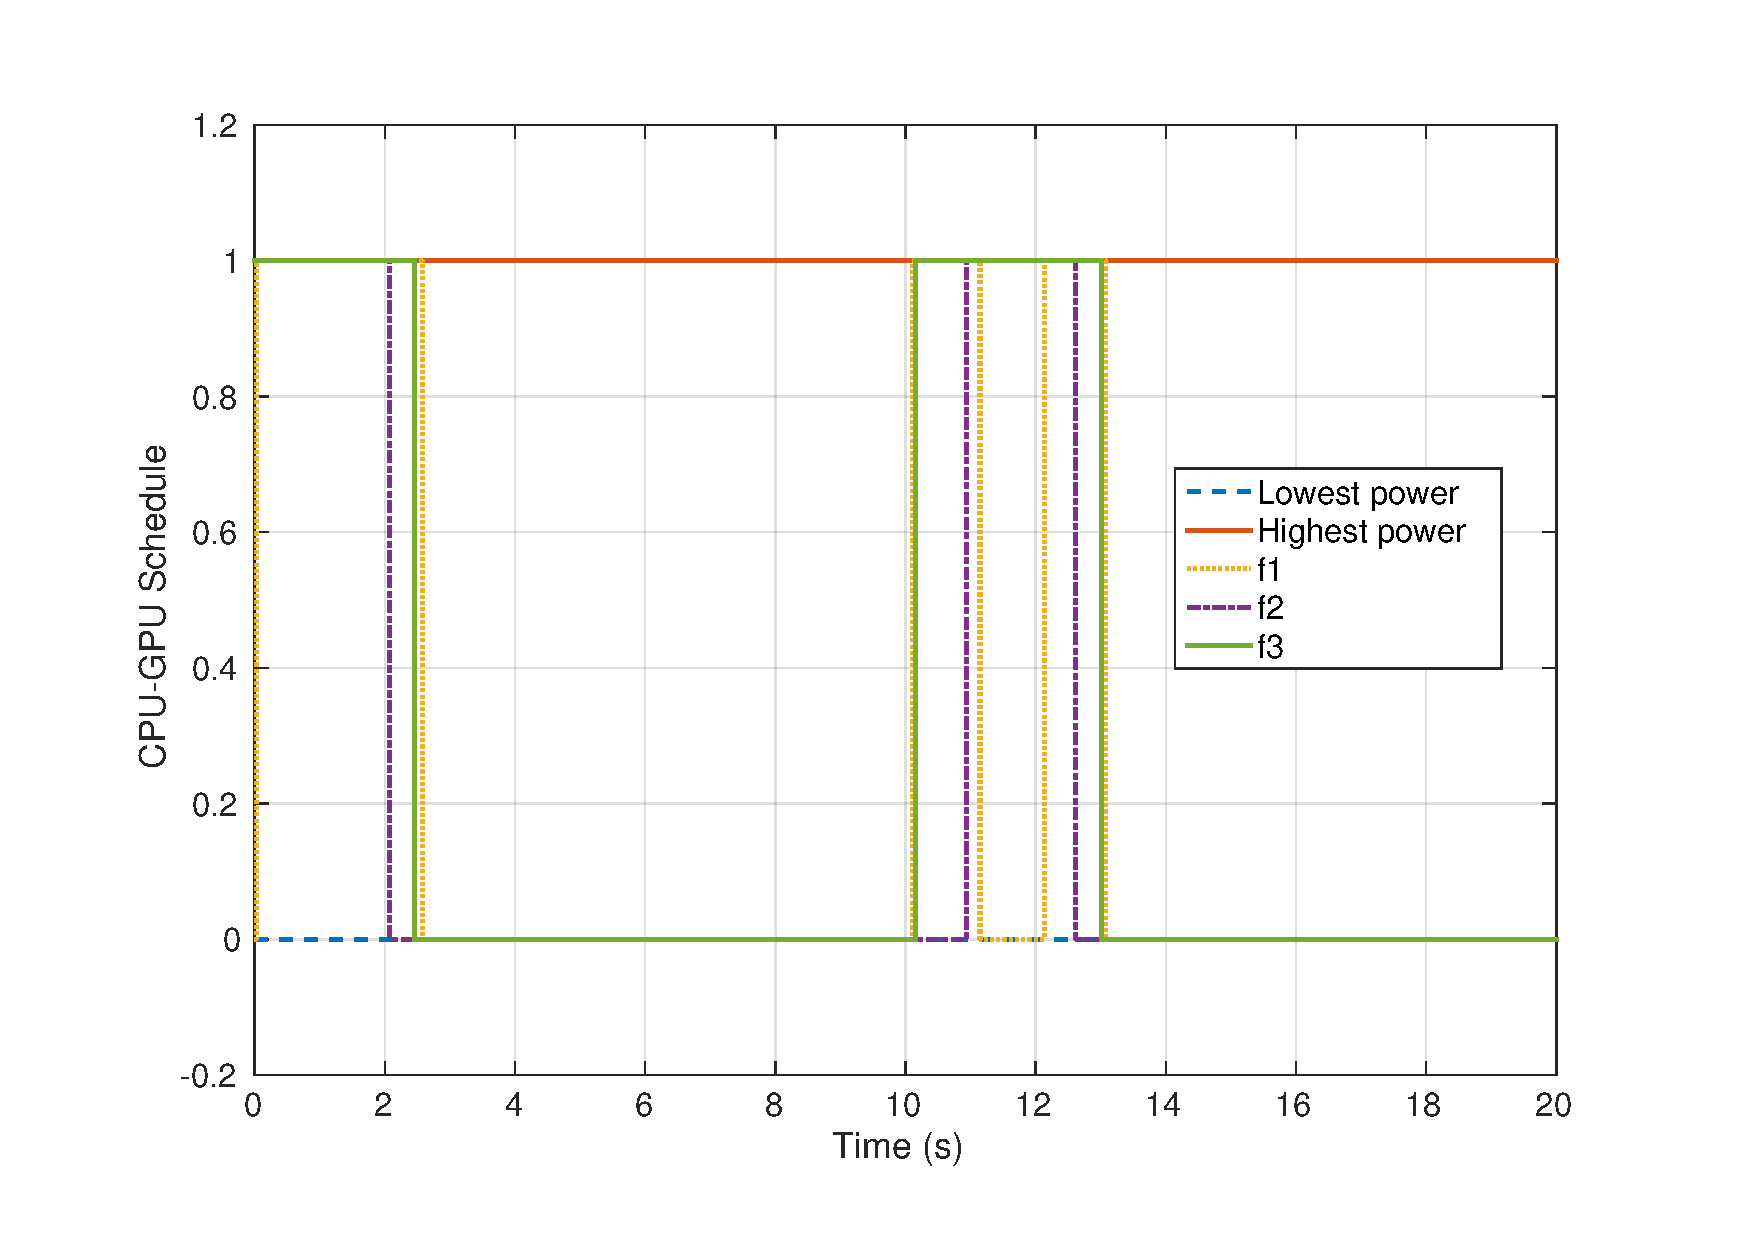
\includegraphics[width=0.49\textwidth]{../simulations/figs/schedule.pdf}
\caption{Resource allocation schedule for the vanishing point algorithm. Note, the schedule switches between only two allocations. This is because the allocation $\alpha=CCG$ has the best throughput while having a relatively low power consumption, while $\alpha=CCC$ has the lowest power consumption. See the results in section \ref{sec:profiling} to get a better idea.}
\label{fig:schedule} 
\end{figure}

\begin{figure}[hbtp]
\centering
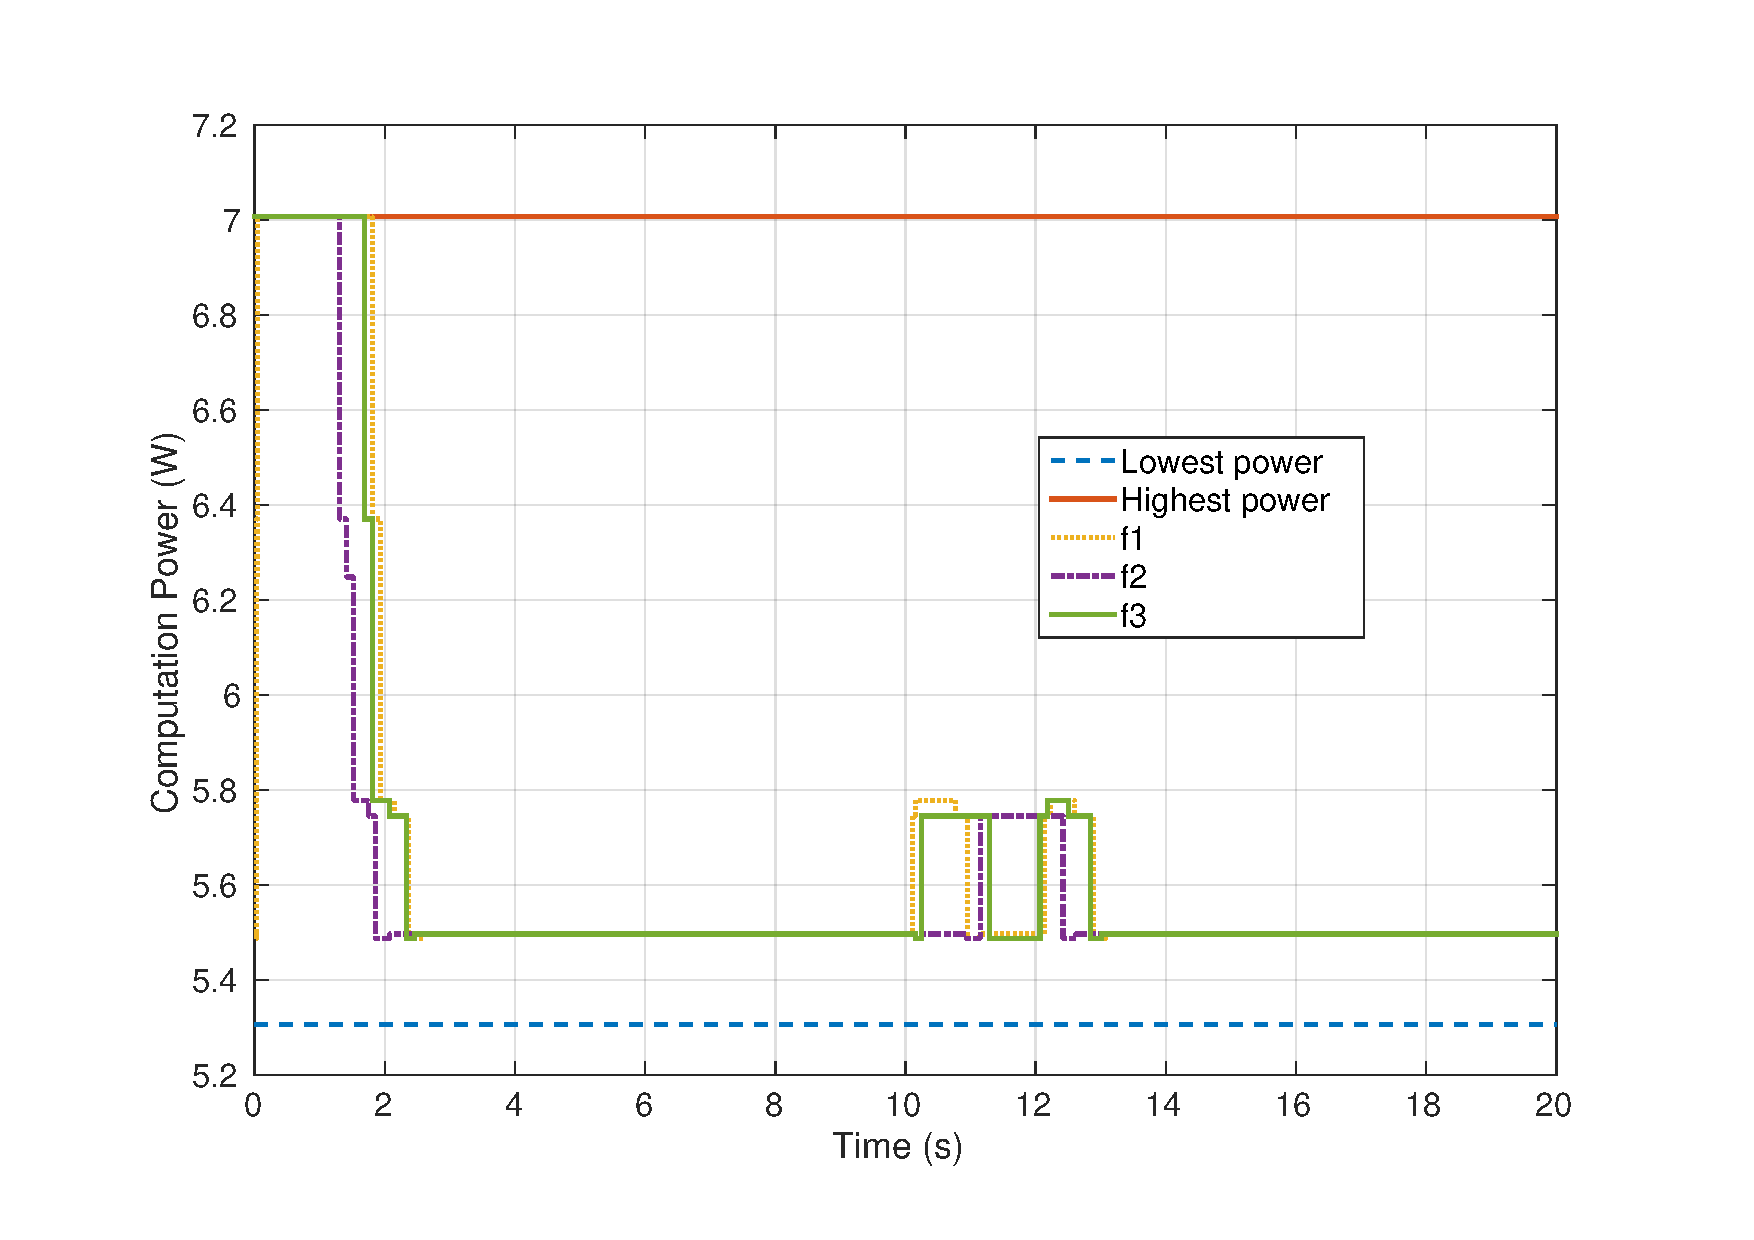
\includegraphics[width=0.49\textwidth]{../simulations/figs/power.pdf}
\caption{Expected computation power for running the vanishing point on the Jetson.}
\label{fig:power} 
\end{figure}






A summary of the control performance and computation energy consumed for these five cases is shown in table \ref{tbl:performance}. It is clear that operating with the highest power/lowest delay mode for the vanishing point results in the best control performance, but the computation energy is high. On the other hand, lowest power/highest delay mode results predictably in low power consumption and the worst control performance. With out two stage approach, control performance is very similar (less than $1\%$ degradation) to the highest power mode, while the computation energy is significantly (about $20\%$) lower. This clearly shows the benefit of our approach.

\begin{table}[htb]
\begin{center}
\caption{Control performance and computation energy}
\label{tbl:performance}
\begin{tabular} {|c|c|c|}
	\hline
	\textbf{Supervisor} & \textbf{Control perf.}(L) & \textbf{Energy}(J) \\ \hline
	Lowest power (mode fixed) & 0.3245 & 106.12  \\ \hline
	Highest power (mode fixed) & 0.3010 & 140.13  \\ \hline
	 $f_1(x_v)$ & 0.3025 & 113.16  \\ \hline
	 $f_2(x_m)$ & 0.3023 & 112.39 \\ \hline
	 $f_3(x_v,x_m)$ & 0.3018 & 113.07 \\ \hline
	 
\end{tabular}
	\vspace{-10pt}	
	\end{center}
\end{table}


